\chapter{Конструкторская часть}

В данном разделе будет приведеная схема последедовательного алгоритма обратной трассировки лучей, а также схемы главного и рабочего потока для параллельной реализации этого алгоритма.

\section{Схема последовательного алгоритма трассировки лучей}

На рисунке \ref{fig:trass_simple} приведена схема последовательного алгоритма трассировки лучей.

\begin{figure}[h!]
	
	\centering{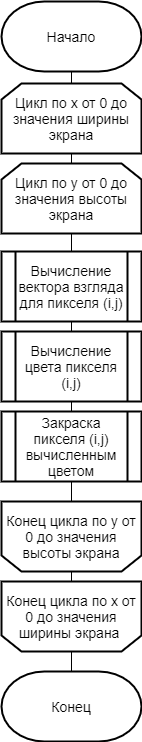
\includegraphics[scale=0.7]{inc/img/trass_simple.png}}
	
	\caption{Схема последовательного алгоритма трассировки лучей}
	
	\label{fig:trass_simple}
	
\end{figure}

\section{Схема параллельного алгоритма трассировки лучей}

На рисунке \ref{fig:trass_split} приведена схема главного потока для параллельной реализации алгоритма трассировки лучей, который разбивает экран на вертикальные участки.

\begin{figure}[h!]
	
	\centering{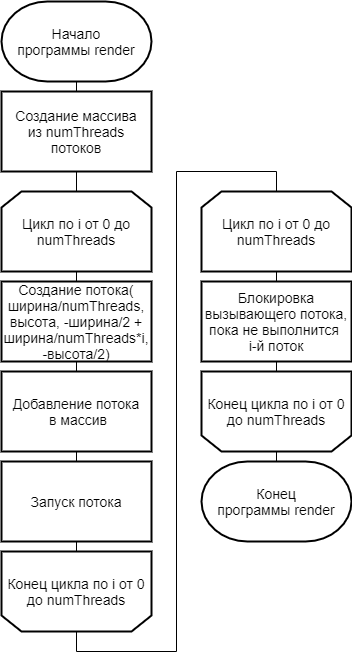
\includegraphics[scale=0.7]{inc/img/trass_split.png}}
	
	\caption{Схема главного потока}
	
	\label{fig:trass_split}
	
\end{figure}

На рисунке \ref{fig:trass_count} приведена схема рабочего потока для параллельной реализации алгоритма трассировки лучей.

\begin{figure}[h!]
	
	\centering{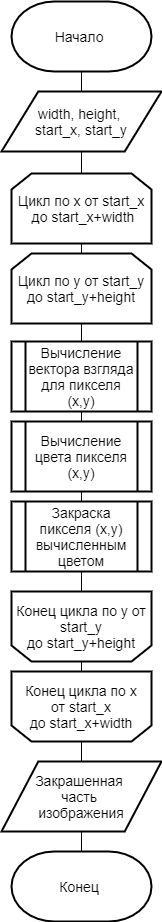
\includegraphics[scale=0.7]{inc/img/trass_count.png}}
	
	\caption{Схема рабочего потока}
	
	\label{fig:trass_count}
	
\end{figure}



\section*{Вывод}

Были разработаны схемы базового и параллельного алгоритмов обратной трассировки лучей.


